% !TEX root = ../main.tex

\chapter{单卡场景下的系统设计与数据路径优化}

\section{单卡系统需求与总体架构}

在完成第三章的任务建模、数据准备和 FlashTOD 执行流程设计之后，本节将研究重点进一步转向系统实现层面，即在单 GPU 条件下，如何通过合理的数据路径组织与执行链路压缩，使异常检测系统在保证检测效果的前提下获得更高吞吐率和更低延迟。单卡场景在本文中具有两层作用：一方面，它是多 GPU 扩展的前提，只有单卡链路本身足够高效，多卡扩展才有现实意义；另一方面，它更容易把系统瓶颈完整地暴露出来，尤其是 CPU$\leftrightarrow$GPU 数据交换、候选结果组织、I/O 等待与算子同步之间的连锁影响。

从系统需求出发，单卡异常检测系统需要同时满足三个目标：在有限显存条件下稳定处理大规模输入，并通过合适的批处理组织支撑候选召回与异常评分连续执行；尽量减少 CPU 对数据平面的直接介入，使查询特征、候选结果与评分中间张量更多停留在 GPU 一侧；在存在外存访问或多阶段流水线的条件下，尽可能重叠 I/O 与 GPU 计算，压缩串行等待时间。由此可见，单卡优化的重点是围绕 GPU 构建一条中间结果传递成本更低的端到端执行链路。

基于这一目标，本文将单卡系统划分为五个核心模块：数据接入与预处理模块、查询向量组织模块、候选召回模块、异常评分模块以及结果输出与日志模块。它们分别承担原始金融记录接入与字段规范化、统一设备侧查询表示构造、候选集合高吞吐返回、候选集上的张量化评分以及最终结果回传与运行时记录等职责。这样的模块划分把热路径和边界路径区分开来：前四个模块构成候选召回到异常评分的核心执行链路，最后一个模块只在必要边界与主机交互。系统总体设计调整之后，能够使系统围绕 GPU 主导路径重新组织它们的衔接关系，避免让这些模块继续沿用``CPU 预处理---GPU 检索---CPU 整理---GPU 评分''的分段模式。

从执行结构上看，本章所研究的单卡系统并不把 FlashANNS 和 PyTOD 当作两个彼此独立的程序，而是把它们放在同一条执行链路的前后两段：前者负责高吞吐候选召回，后者负责精细异常评分，二者之间通过设备侧中间结果表达和统一接口进行衔接。后续各节将围绕这一思路展开，先分析原始链路中的主要瓶颈，再给出 GPU 主导的端到端执行链路，并进一步借助 RAPIDS、FAISS-GPU、pinned memory、异步 stream 和双缓冲等机制对单卡系统做系统性优化。

图~\ref{fig:single-gpu-arch} 展示了单卡系统五个核心模块的连接关系，为后续按数据路径逐层展开分析提供了整体视角。

\begin{figure}[!htbp]
  \centering
  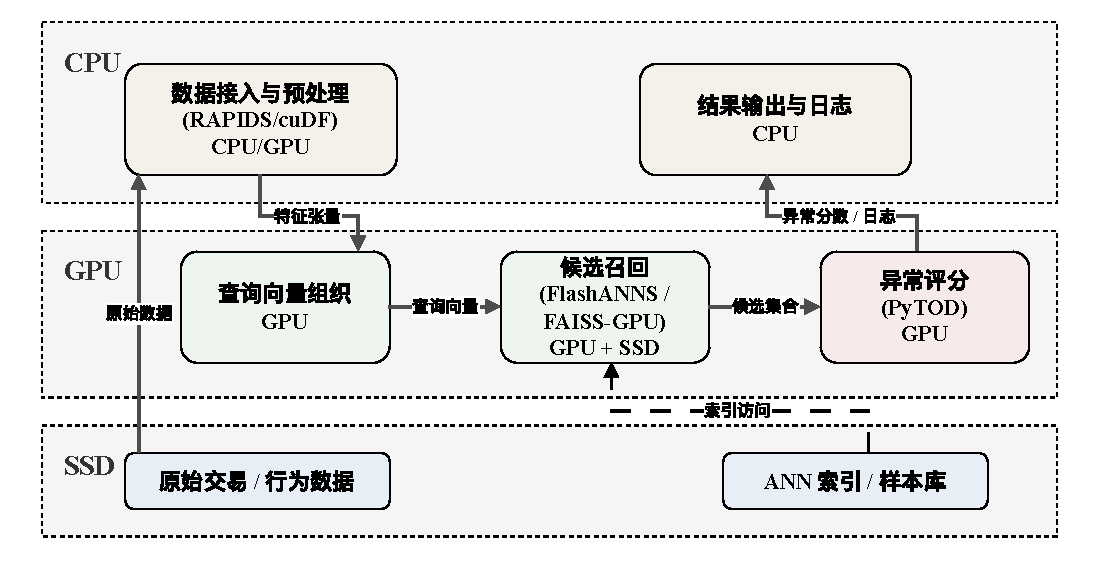
\includegraphics[width=\linewidth]{figures/fig4-1_single_gpu_system_architecture.pdf}
  \caption{单卡异常检测系统总体架构图}
  \label{fig:single-gpu-arch}
\end{figure}

\section{单卡场景下的瓶颈分析}

尽管第三章已经完成了 FlashTOD 执行流程的构建，但从系统执行效率看，原始链路仍存在明显瓶颈。问题在于这些阶段的衔接方式仍然保留了典型的``CPU 主导分段执行''特征：查询特征多在 CPU 侧整理，候选结果在 GPU 上产生后又返回 CPU 重组，后续异常评分再重新依赖 GPU。这样一来，原本分散在不同阶段边界上的开销会在 FlashTOD 链路中叠加出现：传输代价增加，同步点变多，等待时间也被层层放大。

首先，主机与设备之间的频繁边界交换会削弱候选召回和异常评分的单点加速收益。GPU 索引既可接收 host 指针，也可接收 device 指针；当输入本来就在与索引相同的 GPU 上时，不发生拷贝且速度最快，否则会发生 CPU$\rightarrow$GPU 或跨设备拷贝，结果也会在完成后返回相应位置。这意味着，如果查询特征在 CPU 侧完成拼接和标准化，再逐批传输到 GPU，那么即便 GPU 检索本身很快，整条链路仍要持续承担入口传输成本。若候选结果又在 GPU 侧生成后回到 CPU 被重新整理，再送入 PyTOD 评分，则一次查询实际上会跨越两轮主机---设备边界。这样形成的折返路径在小规模实验中未必突出，但在百万级输入和高并发场景下会迅速累积，成为系统瓶颈。

其次，候选中间结果的表达方式会继续放大链路成本。候选召回模块返回的通常不仅是候选样本 ID，还可能包含局部距离、索引位置或局部排序信息。若这些结果优先被组织成 CPU 侧更容易解释的数据结构，例如 Python 对象列表、pandas DataFrame 或主机侧稀疏结构，则后续 PyTOD 在 GPU 上评分前还需要重新完成设备侧重建。这样带来的问题不仅是一次额外的数据复制，更在于它打断了 GPU 对中间张量的连续访问与批量组织能力。因此，在单卡系统中，候选结果若不能以设备侧友好的形式表达和传递，评分阶段就很难形成低开销的连续执行链路。

再次，当候选召回需要访问外存或已经存在明显 I/O 压力时，SSD-I/O 与 GPU 计算之间的串行等待会把前两类问题进一步放大。传统 out-of-core ANN 系统的主要问题之一在于 SSD 访问与 GPU 计算无法有效重叠，系统被迫在``读数据---等数据---算数据''的节奏中推进，从而使高性能 GPU 长时间等待 I/O 完成。而在本文的 FlashTOD 链路中，如果检索内部已经开始重叠 I/O 与计算，但候选召回结束后仍要回到 CPU 完成数据组织和评分前准备，那么被检索阶段隐藏掉的一部分等待会在后续边界重新出现。也正因为这些开销是串联叠加的，单卡优化不能只依赖某一个模块的局部加速，而必须从端到端执行链路出发识别瓶颈。

最后，内存分配与资源组织方式也会在单卡环境下引入隐式开销。\texttt{StandardGpuResources} 会预先保留 scratch memory，以避免频繁 \texttt{cudaMalloc/cudaFree} 导致的同步和性能恶化；页锁定主机内存与内存池机制也有助于稳定传输并减少分配抖动。这说明，即便查询路径和候选结果传递已经更多地留在 GPU 侧，如果系统仍在热路径中频繁申请和释放临时缓冲区，也会因为资源管理本身而造成明显损失。

基于上述分析，本文将单卡场景下的瓶颈概括为四类：查询与候选结果跨边界传递过于频繁、候选中间结果依赖主机侧重组、SSD-I/O 与 GPU 计算之间存在串行等待，以及内存与资源管理带来的隐式同步。这四类问题并不是彼此孤立存在的，它们共同说明单卡系统要获得稳定收益，关键在于压缩整条数据路径。

图~\ref{fig:baseline-bottlenecks} 以并列方式对比了原始 CPU$\leftrightarrow$GPU 往返链路与优化后的 GPU 主导连续链路，直观说明多次 H2D/D2H 传输和阶段同步如何成为主要瓶颈；表~\ref{tab:single-gpu-bottlenecks} 则对这些瓶颈的类型与后续优化方向进行了分类。

\begin{figure}[!htbp]
  \centering
  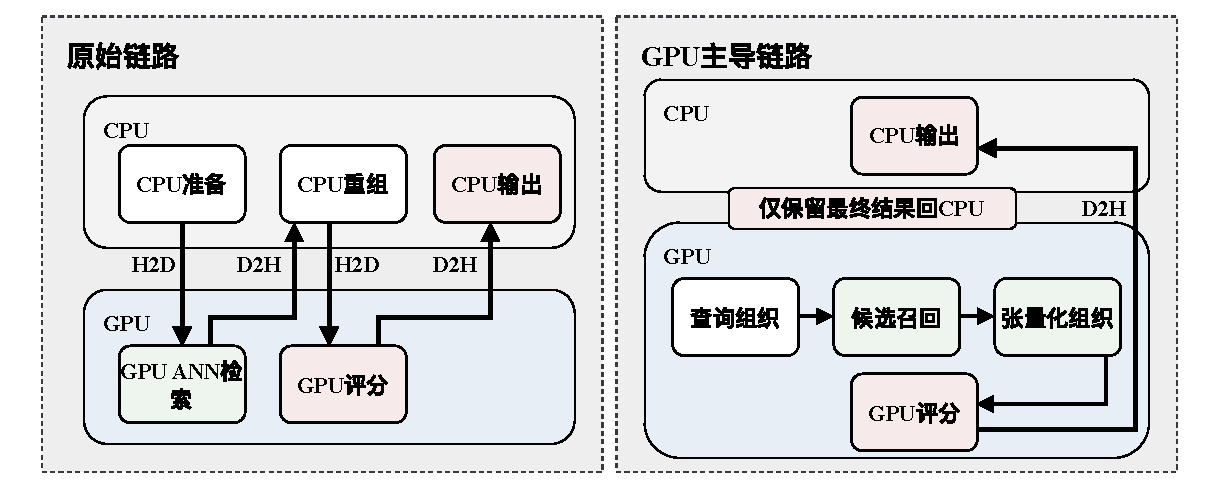
\includegraphics[width=\linewidth]{figures/fig4-2_original_vs_gpu_dominant_chain.pdf}
  \caption{原始链路与 GPU 主导链路对比图}
  \label{fig:baseline-bottlenecks}
\end{figure}

\begin{table}[htbp]
  \caption{单卡主要瓶颈与对应优化项}
  \label{tab:single-gpu-bottlenecks}
  \centering
  \footnotesize
  \setlength{\tabcolsep}{2.8pt}
  \renewcommand{\arraystretch}{1.20}
  \begin{adjustbox}{max width=0.98\linewidth}
    \begin{tabular}{P{1.75cm}P{1.95cm}P{2.15cm}P{2.65cm}P{2.95cm}P{2.95cm}}
      \toprule
      瓶颈类型 & 发生位置 & 主要影响 & 对应优化方案 & 涉及组件 & 预期收益 \\
      \midrule
      高频 CPU$\leftrightarrow$GPU 往返 &
      查询准备、候选输出与评分结果边界 &
      放大 H2D/D2H 次数，增加同步等待与尾延迟 &
      GPU 主导执行链路，边界处结合 pinned memory 做必要交换 &
      \makecell[l]{RAPIDS/cuDF\\PyTOD\\RMM pinned\\memory} &
      \makecell[l]{降低跨设备往返频次，\\压缩尾延迟并提高\\端到端吞吐} \\
      \midrule
      候选重组开销 &
      候选召回到异常评分的接口边界 &
      主机侧 pack\_candidates、序列化和重建成本高 &
      采用设备常驻候选缓冲（device-resident candidate buffer）和统一张量交接接口 &
      \makecell[l]{FlashANNS\\FAISS-GPU\\PyTOD} &
      \makecell[l]{缩短候选打包阶段，\\避免 CPU 重新成为\\数据平面瓶颈} \\
      \midrule
      I/O 串行等待 &
      SSD 读页、ANN 图扩展与局部距离计算之间 &
      GPU 空转等待数据，召回吞吐受限 &
      异步 I/O 重叠、双缓冲和流级并行推进 &
      \makecell[l]{FlashANNS\\NVMe SSD\\CUDA streams} &
      \makecell[l]{隐藏部分读页等待，\\提高候选召回有效吞吐\\与 GPU 忙碌度} \\
      \midrule
      资源分配抖动 &
      临时缓冲区、scratch memory 与主机交换缓冲 &
      频繁分配释放导致延迟抖动和显存碎片 &
      内存池复用、scratch 预分配与微批双缓冲 &
      \makecell[l]{FAISS\\\texttt{GpuResources}\\RMM memory\\pool\\CUDA streams} &
      \makecell[l]{稳定阶段延迟，降低\\分配开销（allocation\\overhead），改善资源利用率} \\
      \bottomrule
    \end{tabular}
  \end{adjustbox}
\end{table}

\section{GPU 主导的端到端执行链路设计}

针对上一节所分析的瓶颈，本文设计面向单卡场景的 GPU 主导端到端执行链路。这一路径的核心做法是：在 FlashANNS 提供的异步 I/O---计算流水线基础上，把查询特征组织、候选检索结果传递与异常评分中间张量计算尽量收拢到 GPU 一侧，仅在必要边界通过页锁定内存等机制完成主机交互，从而同时压缩 SSD-I/O 与 GPU 计算之间的串行等待，以及主机---设备边界上的额外搬运。

从总体原则上看，GPU 主导端到端执行链路包含三层含义：查询特征的最终组织尽可能在 GPU 侧完成；候选召回结果以设备侧可直接消费的形式交给异常评分模块；评分阶段产生的中间张量继续在设备侧推进，只有最终分数、排序结果或必要日志信息再回传 CPU。对应到系统行为上，这一路径的真正收益并不是某一次传输被完全消除，而是把原先反复出现的``主机---设备---主机---设备''折返模式压缩为少数必要边界交互。

\subsection{查询特征在 GPU 侧的驻留与组织}

在原始实现中，金融交易数据通常先以表格形式在 CPU 侧完成清洗、归一化和拼接，再整体打包为查询向量传入 GPU。这样组织虽然直观，但会让所有查询都在入口处承担一次完整的 H2D 成本。本文在这一位置的设计决策，是把部分预处理与特征组织前移到 GPU 数据处理后端，使关键查询向量尽可能在设备侧形成最终表示。RAPIDS 的 GPU DataFrame 组件 cuDF，以及与其协同的 GPU 数组计算库 CuPy，提供了批量列运算、张量表达和统计聚合能力，使这一做法在工程上具备可行性\citep{rapids_cudf_pandas}。预期收益也较为直接：查询入口不再承担整批向量的重复搬运，后续候选召回阶段能够更快接收到可检索的设备侧表示。

\subsection{候选检索结果在 GPU 侧的保持与传递}

候选召回阶段结束后，系统面临的关键问题是：候选结果应以何种形式进入异常评分模块。本文在这里的设计决策，是尽量保持候选结果为设备常驻（device-resident）对象，即候选 ID、局部距离和必要索引信息不先回 CPU 再重建，而是在 GPU 上直接组织为 PyTOD 可消费的中间张量。FAISS-GPU 文档指出，同 GPU 上的输入与输出可以避免额外拷贝，且 \texttt{GpuResources} 可通过预分配 scratch memory 降低中间缓冲区分配开销\citep{faiss_gpu_wiki}。沿着这一接口设计，FlashANNS/FAISS-GPU 的输出可以自然流入 PyTOD 评分阶段的设备侧对象，预期收益主要体现在候选打包和阶段切换成本的下降。

\subsection{异常评分中间张量的 GPU 常驻执行}

PyTOD 评分阶段本身具备张量化执行基础，因此在本文设计中，其主要中间表示包括候选距离矩阵、局部排序结果、聚合统计量和最终异常分数。本文在这一位置的选择很明确：中间张量不在计算过程中回到 CPU，而是在 GPU 上连续推进，直到得到最终小规模输出后再按需回传主机。这样做的原因在于，一旦这些对象中途离开 GPU，不仅会增加 D2H 成本，还会破坏 PyTOD 在设备侧连续执行和批量算子复用的优势。预期收益因此不仅表现为传输减少，也表现为评分阶段的局部性和算子复用被更好地保留。

\subsection{必要条件下的主机侧交互与页锁定内存机制}

GPU 主导执行并不意味着 CPU 在单卡系统中完全消失。原始输入读取、部分日志写回、结果落盘以及特定部署场景下的主机接口，仍然要求系统与 CPU 保持交互。因此，这一小节对应的设计决策不是“取消主机交互”，而是把交互严格限制在必要边界，并通过页锁定内存等机制把这些边界开销控制在较低水平。RMM 文档指出，\texttt{PinnedHostMemoryResource} 可提供页锁定主机内存，从而加快 Host$\leftrightarrow$Device 数据传输\citep{rapids_rmm_pinned}。这类机制的收益主要不是提高某个算子的峰值速度，而是降低必要交互对整条热路径的干扰。

因此，单卡热路径只保留必要的主机边界：查询向量、规范化特征、候选 ID/distance/rank 以及 PyTOD 的距离矩阵、排序和聚合张量尽量在 GPU 侧连续传递；原始输入、最终异常分数和运行日志则以小规模方式回到 CPU。这样既保留系统可观察性，也避免候选到评分之间重新形成主机侧折返。

\section{基于 FlashANNS 的异步 I/O---计算流水线融合}

在上一节确立 GPU 主导执行链路之后，本节进一步处理另一类关键问题：如何把候选召回阶段内部的 I/O 等待压缩到最低，并使这种收益真正传导到系统整体。FlashANNS 的设计表明，传统 out-of-core 检索系统存在明显的串行等待特征；而通过依赖放松异步流水线（dependency-relaxed asynchronous pipeline），可以使 I/O 和 GPU 计算在更大程度上重叠，从而提升候选召回吞吐\citep{xiao2025flashanns}。本文在单卡系统中继续把它与 GPU 主导执行链路衔接起来，使检索内部收益不会在后续阶段被新的边界开销抵消，避免简单地把这一路径嵌进去。

具体而言，系统在候选召回阶段不再将 SSD-I/O 视为必须先完成的前置步骤，而是把检索中的部分访问与 GPU 侧局部计算、候选维护和评分前准备并行组织。对检索内部而言，这意味着查询在等待部分图节点或向量块从 SSD 到达时，GPU 仍可继续推进已到达部分的距离计算和候选维护；对本文系统整体而言，这意味着候选召回阶段的等待不再以完整停顿的形式暴露在评分入口前，而是更多地被吸收到设备侧持续运行的流水线中。

这一融合的收益主要表现在两个层面。对 FlashANNS 内部而言，候选召回阶段的有效吞吐被提高，GPU 不再频繁因为等页到达而空转；对本文系统整体而言，PyTOD 评分模块不需要周期性等待检索阶段完全结束才能获得候选输入，能够更连续地获得候选输入。更重要的是，由于候选结果继续保留在 GPU 一侧，中间结果不必回到 CPU 侧整理，FlashANNS 内部获得的 I/O---计算重叠收益也不会在后续阶段被新的边界阻塞抵消。

从实现角度看，这一融合要求系统在单卡场景下对流、缓冲区和中间结果表达进行统一组织，而FlashANNS 对 warp 级并发 SSD 访问和双缓冲思想的使用，也支持这种边访问边计算的路径可以落到具体执行机制上的\citep{xiao2025flashanns}。

图~\ref{fig:io-compute-integration} 展示了 FlashANNS 异步流水线与本文链路的融合方式。

\begin{figure}[!htbp]
  \centering
  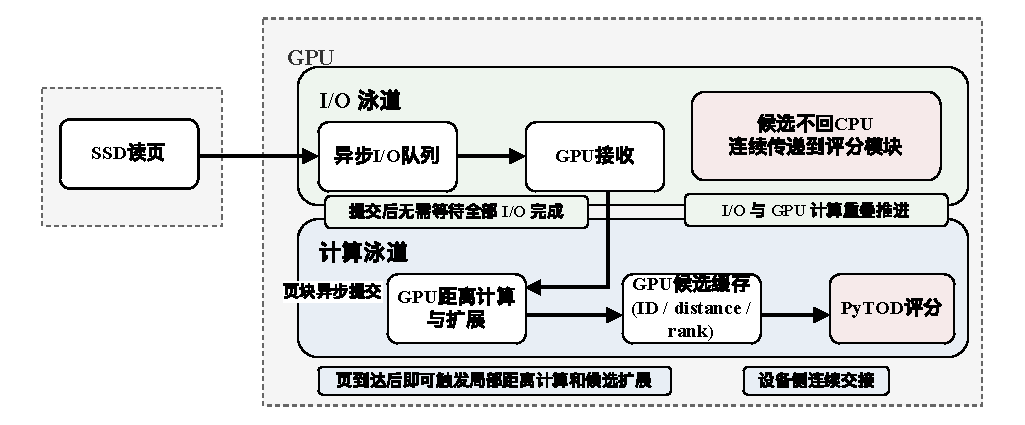
\includegraphics[width=\linewidth]{figures/fig4-3_flashanns_async_io_compute_pipeline.pdf}
  \caption{FlashANNS 异步 I/O---计算流水线与本文执行链路融合}
  \label{fig:io-compute-integration}
\end{figure}

这一链路把 SSD 读页等待、页到达后的局部计算和批次切换尽量交叠起来：异步 I/O 队列削弱等待，warp 级并发访问与双缓冲候选缓存维持设备侧连续推进，候选结果则直接进入评分模块，避免重回 CPU 打包。

\section{数据处理与计算后端优化}

在完成 GPU 主导执行链路和 FlashANNS 异步流水线融合之后，单卡系统仍需要进一步优化数据处理与计算后端，以减少表格型中间结果处理和设备资源管理所带来的额外开销。为此，本文在原始 PyTorch/CPU 数据路径基础上引入 RAPIDS 体系，对金融数据预处理、特征拼接、中间结果组织和批量统计环节进行后端重构\citep{rapids_cudf_pandas,rapids_rmm_pinned}。

后端优化围绕热路径展开：字段筛选、类型转换和窗口统计尽量前移到 RAPIDS/cuDF；候选组织、批量拼接和统计聚合转为 GPU DataFrame 或 CuPy 张量表达；临时内存与必要的主机交换缓冲由 RMM 内存池和页锁定主机端（pinned host）资源管理；与 PyTOD、检索后端交接时，则优先采用设备侧连续缓冲，避免``DataFrame---Python 对象---Tensor''的反复转换路径\citep{rapids_rmm_pinned}。

由此，RAPIDS 在本文中并不是替代检测算法，而是用于稳定热路径的数据和内存后端。后端重构的直接目标，是缩短 query\_prep、pack\_candidates 以及检索资源初始化中的对象转换和资源抖动。

\section{候选检索后端优化}

除了数据处理后端的重构外，候选检索后端本身也需要进一步工程化优化。虽然 FlashANNS 提供了高吞吐候选召回机制，但在实际系统实现中，检索后端不仅要关注检索内部的吞吐，还要关心查询输入、候选输出以及评分模块之间的接口组织是否会重新引入边界成本。FAISS-GPU 在这方面提供了成熟的工程支撑，其主机/设备指针（host/device pointer）互操作、资源对象管理和多种 GPU 索引形式，使其适合作为本文系统中的候选检索后端增强组件\citep{faiss_gpu_wiki}。

本文在检索后端上的优化主要体现在三个方面：统一检索输入接口，使查询向量能够以设备侧对象直接进入检索后端，避免不同检索组件对输入格式提出不同要求；统一候选输出接口，使 FlashANNS 或 FAISS-GPU 返回的候选结果都能以 GPU 侧张量形式被 PyTOD 消费，从而减少后端切换带来的中间转换；统一资源管理策略，通过 FAISS 的 \texttt{GpuResources} 与系统侧缓冲区管理配合，降低临时缓冲区申请和释放频率，稳定检索阶段的延迟与吞吐表现\citep{faiss_gpu_wiki}。这些优化的共同目标，是让检索后端更顺畅地嵌入整条热路径，避免单独追求某个后端组件的峰值性能。

\section{单卡执行链路的工程增强}

在完成数据路径、异步流水线和后端优化后，系统仍然需要若干工程增强机制来保证单卡链路在高负载下保持稳定。这些增强能够补足其稳定性与可观察性，包括异步 CUDA stream 组织、双缓冲与微批执行、显存碎片控制以及日志和性能采样机制。

在流组织方面，本文通过将查询准备、候选检索、评分计算和必要的主机边界交互映射到不同 CUDA stream，使数据传输、检索和评分能够在更大程度上并行推进。在缓冲方面，本文采用双缓冲与微批组织方式：当当前批次进入候选召回与评分阶段时，下一批次的输入组织和部分准备可以并行进行，从而进一步压缩流水线空泡。在显存管理方面，本文通过限制中间张量生命周期、统一缓冲区尺寸以及使用内存池机制减少碎片和反复分配开销。在监控与可观察性方面，本文建立统一日志字段与性能采样机制，记录查询输入规模、候选集合规模、各阶段耗时、GPU 利用率和 Host$\leftrightarrow$Device 交互次数，为后续章节分析多 GPU 扩展提供统一观测基础。

\section{单卡实验与性能分析}

为了验证前述单卡系统设计与数据路径优化的有效性，本文将单卡实验口径统一组织为“真实集 $\rightarrow$ 1M 合成数据 $\rightarrow$ 10M 合成数据 $\rightarrow$ 50M 合成数据”。其中，真实集用于保持与方法有效性验证一致的现实口径，1M 合成数据承担由真实集过渡到系统实验的桥接角色，10M 与 50M 合成数据对应单卡性能分析的主体规模。在这一框架下，本节重点比较四类方案：原始分段执行链路、仅启用候选召回加速的链路、启用 GPU 主导执行链路但不做后端重构的链路，以及本文完整的单卡优化方案。这样的对比口径能够区分不同收益来源：候选召回本身带来的收益、执行链路重构带来的收益，以及后端与工程增强叠加后的整体收益。换言之，这四类方案构成递进式消融实验，用于观察候选召回、数据路径压缩和后端重构在端到端性能中的累积贡献。实验关注的指标包括每秒查询数（Queries Per Second，QPS）、平均延迟与 99 分位延迟（p99 latency，p99）、CPU$\leftrightarrow$GPU 传输次数与体积、GPU 利用率、I/O 利用率以及各阶段耗时分解。

实验结果显示，单纯依赖候选召回加速虽然能够降低部分检索耗时，但若候选结果仍需回到 CPU 侧整理再进入评分，端到端吞吐提升并不充分。相比之下，当查询特征、候选结果与评分中间张量更多地留在 GPU 一侧后，主机---设备边界交互次数明显减少，系统吞吐率和延迟分位数都表现出更稳定的改善。进一步地，当 FlashANNS 的异步 I/O---计算流水线与设备侧连续执行链路结合后，候选召回阶段的等待可以被部分隐藏，评分阶段也更容易连续接收输入，反映在更高的 GPU 利用率上。

从阶段耗时分解来看，优化前系统的主要开销集中在查询组织、候选结果主机侧重组和阶段同步等待；优化后，系统性能不再首先被路径开销拖住，其决定因素开始更多落在 GPU 侧核心阶段，主要耗时更多地集中到设备侧检索与评分本身。

考虑到本节结果展示需要兼顾版面与代表性，图~\ref{fig:single-stage-breakdown} 与图~\ref{fig:single-stage-breakdown-large} 选取 1M 与 10M 两个具有代表性的合成规模展示阶段耗时分解，图~\ref{fig:single-gpu-overview} 汇总比较四种方案在 QPS、p99 延迟、PCIe 传输次数与 GPU 利用率上的综合表现。

\begin{figure}[!htbp]
  \centering
  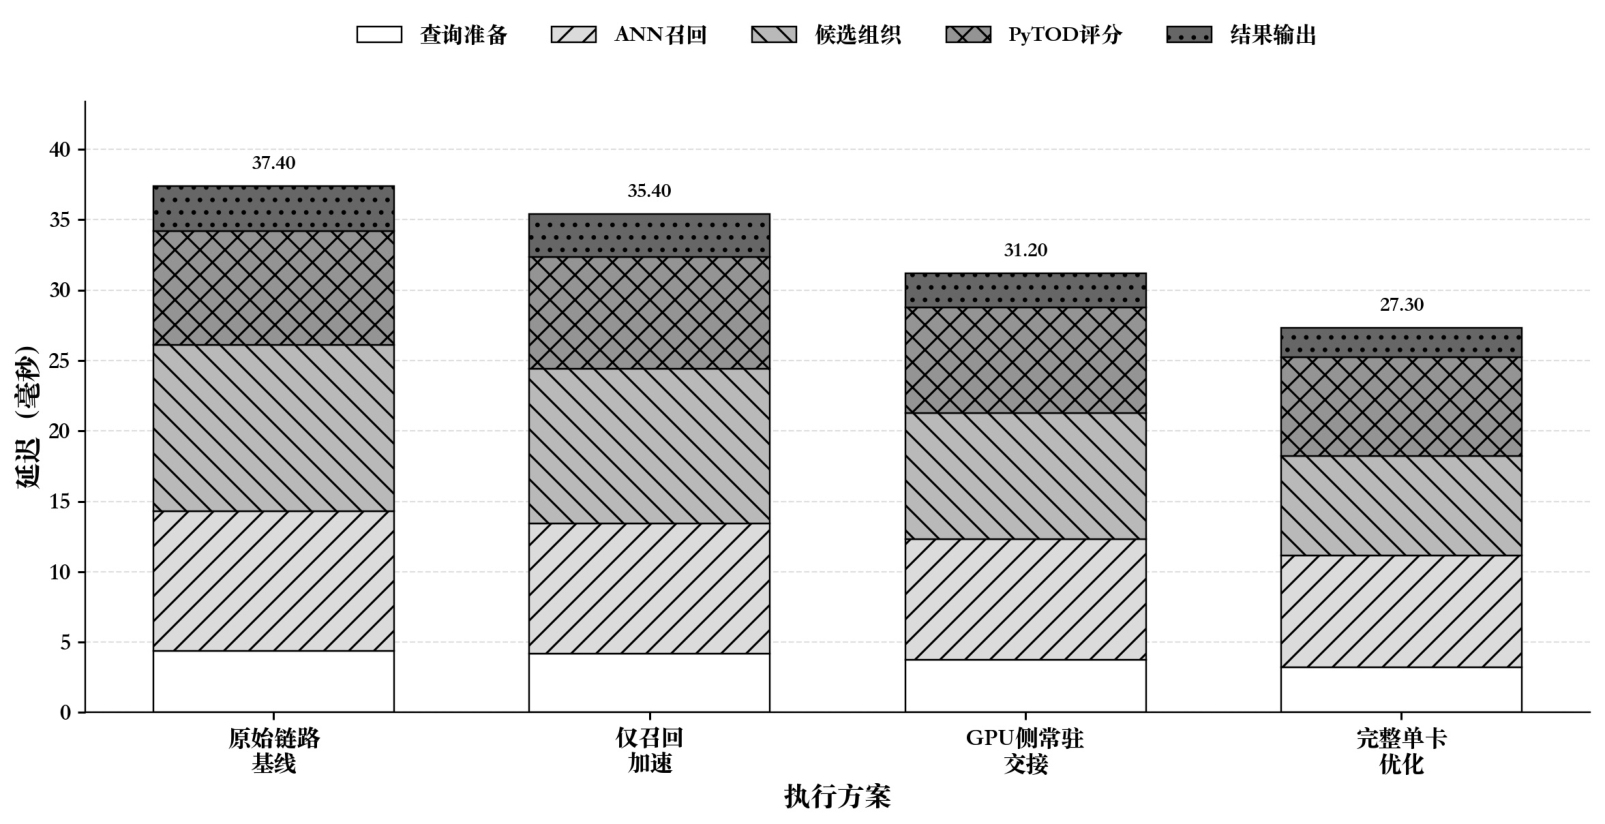
\includegraphics[width=\linewidth]{plot_assets/ch04_single_gpu_stage_breakdown/fig4_14_single_gpu_stage_breakdown_1m.pdf}
  \caption{1M 数据规模下单卡各阶段耗时分解}
  \label{fig:single-stage-breakdown}
\end{figure}

\begin{figure}[!htbp]
  \centering
  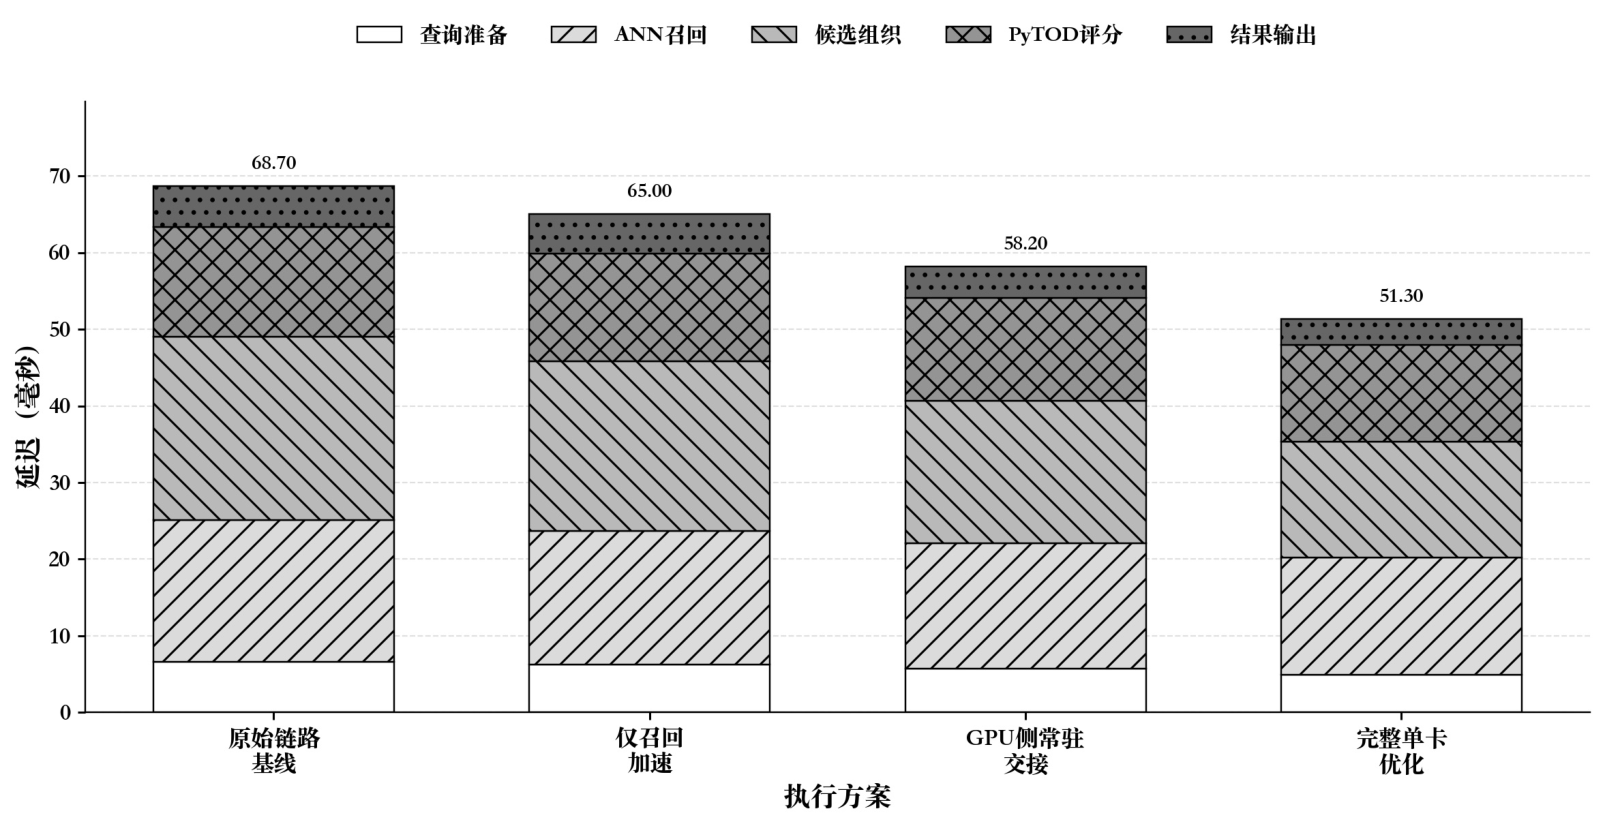
\includegraphics[width=\linewidth]{plot_assets/ch04_single_gpu_stage_breakdown/fig4_15_single_gpu_stage_breakdown_10m.pdf}
  \caption{10M 数据规模下单卡各阶段耗时分解}
  \label{fig:single-stage-breakdown-large}
\end{figure}

\begin{figure}[!htbp]
  \centering
  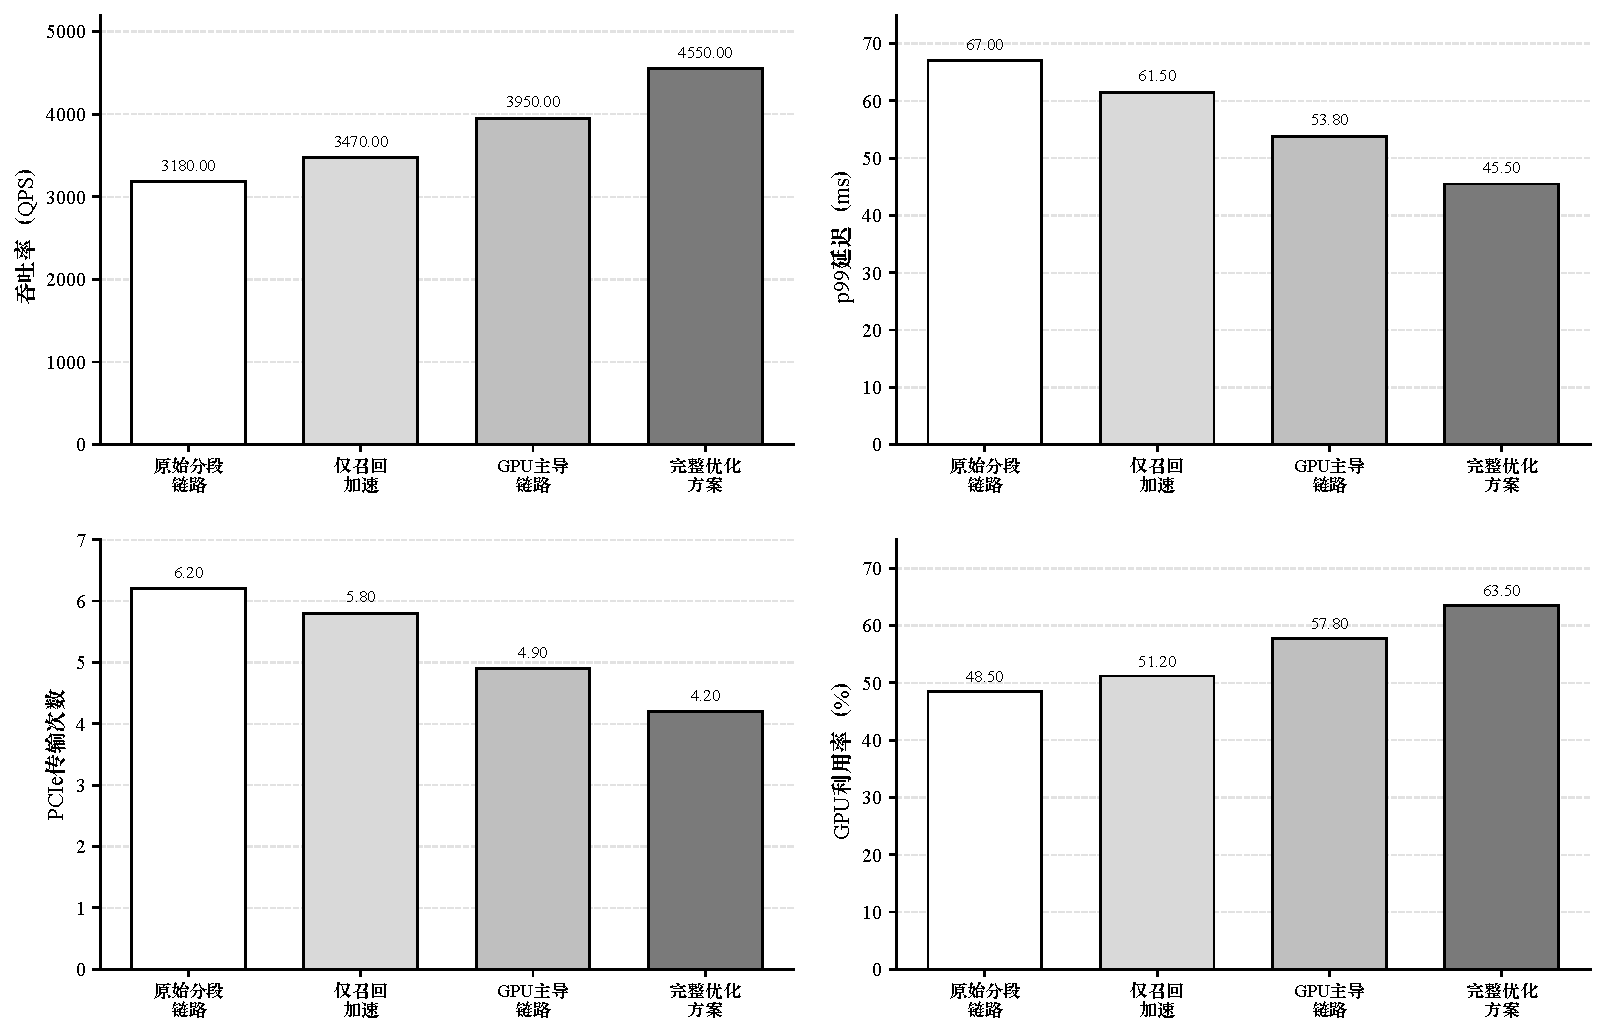
\includegraphics[width=0.95\linewidth]{figures/exp/single_gpu_progressive_ablation.pdf}
  \caption{单卡执行链路递进式消融结果}
  \label{fig:single-gpu-overview}
\end{figure}

图~\ref{fig:single-gpu-overview} 展示的是递进式消融，而不是完全独立的单因素消融。仅启用候选召回后，QPS 有所提高但 p99 延迟和 PCIe 传输次数下降有限，说明召回模块本身并不能消除阶段边界开销；引入 GPU 主导链路后，候选组织和评分输入更多留在设备侧，p99 延迟与传输次数进一步下降；完整优化方案在此基础上叠加后端和资源管理优化，使吞吐、尾延迟和 GPU 利用率同时改善。这一结果说明系统收益主要来自候选召回、数据路径压缩和后端重构的累积作用。

\section{本章小结}

本章围绕单 GPU 场景下的系统实现问题，分析了原始 FlashTOD 链路中存在的边界交换、候选重组、I/O 等待以及资源管理抖动等瓶颈，并在此基础上设计了 GPU 主导的端到端执行链路。围绕这条链路，本文进一步引入 RAPIDS 与 FAISS-GPU 对数据处理与候选检索后端进行工程增强，并通过异步 stream、双缓冲、内存池与统一监控机制补充其稳定性与可观察性。

单卡实验的结果说明，本章的主要收益并不来自某一个局部算子的极限加速，而来自候选召回到异常评分整条数据路径的压缩，以及设备侧连续执行能力的增强。经过这一轮优化后，系统的主要压力已经更多集中到 GPU 侧核心阶段，这也使下一章有必要转向多 GPU 场景：当单卡链路已经被尽量收紧之后，系统吞吐的进一步提升才真正转化为多 GPU 扩展问题。
